\section{Some introductory examples}

The previous chapter considered detection problems where we are given a set of observations and, based on them, we have to infer (decide) which hypothesis is true. Concretely, we have studied how to design the optimal detector (according to some criterion: maximum likelihood, minimum expected cost, etc.) and how to analyze its performance (false alarm and detection probabilities, error probability or average cost). 

In this chapter, we will study a different approach to detection problems, where the observations arrive sequentially and, moreover, we can decide whether we want to acquire more observations to achieve the desired performance. These problems are referred to as sequential detection problems, where the objective is to take a decision as soon as possible (acquiring the smallest amount of observations), while ensuring the required performance. 

In the following, we will study the problem of sequential detection in a simple set-up where there are only two hypotheses whose likelihoods are perfectly known, and the observations are independent and identically distributed (i.i.d.). But before we address the problem in a formal manner, this section presents two simple examples to introduce it. Concretely, we consider examples with and without gathering costs.

\subsection{Example 1: Sequential detection with no gathering cost}

Here, we present a simple example to motivate the problem of sequential detection. Consider an experiment in which the observation at time $n$ under hypothesis $H = 0$ follows a zero-mean Gaussian distribution with variance $\sigma^2 = 1$, and under hypothesis $H = 1$, the observation follows a zero-mean Gaussian distribution with variance $\sigma^2 = 4$. That is, the likelihoods are
\begin{equation}
	\label{eq:likelihood_0}
	p_{X[n] | H} (x[n] | 0) = \frac{1}{\sqrt{2 \pi}} \exp \left(-\frac{x^2[n]}{2}\right),
\end{equation}
and
\begin{equation}
	\label{eq:likelihood_1}
	p_{X[n] | H} (x[n] | 1) = \frac{1}{\sqrt{8 \pi}} \exp \left(-\frac{x^2[n]}{8}\right),
\end{equation}
which are shown in Figure \ref{fig:likelihoods_sequential}. Moreover, we assume that the observations are i.i.d.

\begin{figure}[t]
	\pgfmathsetmacro{\mypi}{3.141592}
	\begin{center}
		\begin{tikzpicture}
			\begin{axis}[%
				axis x line=middle,
				axis y line=middle,
				enlarge x limits=0.05,
				enlarge y limits=0.2,
				% xtick={-\mypi,-2*\mypi/\windowlength,2*\mypi/\windowlength,\mypi},
				% xticklabels={$-\pi$,$-\frac{2\pi}{N}$,$\frac{2\pi}{N}$,$\pi$},
				xmin=-6,
				xmax=6,
				ymin=0,
				%ytick=\empty,
				width=10cm,
				height=7.5cm,
				domain = -6:6,
				samples = 512,
				xlabel={$x[n]$},
				ylabel={$p_{X[n] | H} (x[n] | h) $}]
				\addplot[blue,thick] {1/sqrt(2*\mypi)*exp(-x^2/2)};
				\addplot[red,thick,dashed] {1/sqrt(8*\mypi)*exp(-x^2/8)};
				\legend{$h = 0$,$h = 1$};
			\end{axis}
		\end{tikzpicture}
	\end{center}
	\caption{Likelihoods considered in the introductory example}
	\label{fig:likelihoods_sequential}
\end{figure}

We shall start by considering no observations, $n = 0$, and derive the detector with minimum average cost and its cost. Concretely, considering $c_{00} = c_{11} = 0$ and $c_{01} = c_{10} = 1$, the minimum expected cost detector optimizes the cost
\begin{align*}
	\overline{C}_0 &= \mathbb{E}\{c_{DH}\} \\ &= c_{10} P(D = 1, H = 0) +  c_{01} P(D = 0, H = 1)  + c_{00} P(D = 0, H = 0) +  c_{11} P(D = 1, H = 1)  \\
	&= P(D = 1, H = 0) +  P(D = 0, H = 1) \\ &= P(D = 1 | H = 0) P_H(0) +  P(D = 0 |H = 1) P_H(1)
	\\ &= P(D = 1 | H = 0) p +  P(D = 0 |H = 1) (1 - p),
\end{align*}
where we have defined, for the sake of notation, $P_H(0) = p$ and $P_H(1) = 1 - p$. The probabilities $P(D = 1 | H = 0)$ and $P(D = 0 | H = 1)$ are determined by the detector. However, since there are no observations, the detector must always decide the same hypothesis, making one of the aforementioned probabilities one and the other zero. Then, for $0 \leq p \leq 1/2$, we should always decide $D = 1$, which yields $P(D = 1 | H = 0) = 1$, $P(D = 0 | H = 1) = 0$, and
\begin{equation*}
	\overline{C}_0 = p.
\end{equation*}
If we had decided always $D = 0$, we would have $P(D = 1 | H = 0) = 0$, $P(D = 0 | H = 1) = 1$, and
\begin{equation*}
	\overline{C}_0 = 1 - p,
\end{equation*}
which is obviously larger than $\overline{C}_0 = p$ for $0 \leq p \leq 1/2$. Similarly, for $1/2 < p \leq 1$, we should always decide $d = 0$, which implies that $P(D = 1 | H = 0) = 0$, $P(D = 0 | H = 1) = 1$, and
\begin{equation*}
	\overline{C}_0 = 1 - p.
\end{equation*}
Combining both results, the minimum average cost for varying $p$ is
\begin{equation*}
	\overline{C}_0(p) = \begin{cases} p, & 0 \leq p \leq 1/2, \\ 1 - p, & 1/2 < p \leq 1, \end{cases}
\end{equation*}
where we have explicitly written the dependence of the minimum average cost  with $p$. Figure \ref{fig:average_cost_n0} shows $\overline{C}_0(p)$ for varying $p$.

\begin{figure}[t]
	\begin{center}
		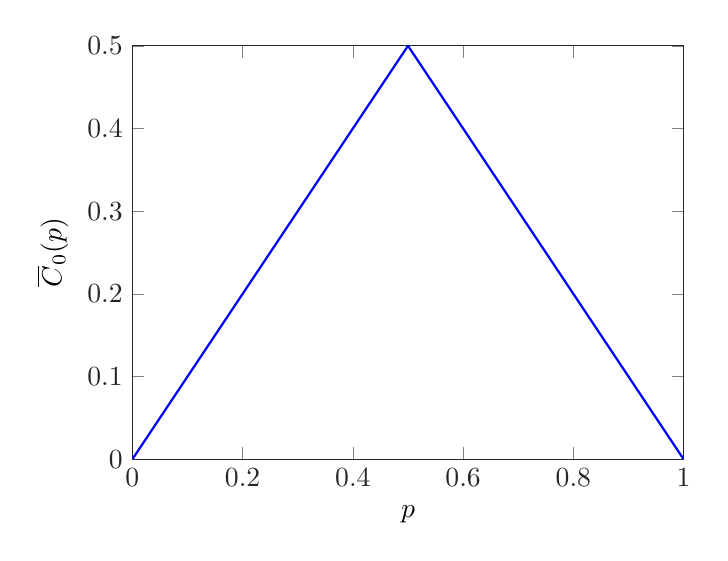
\begin{tikzpicture}
			\begin{axis}[%
				width=7cm,
				height=5.25cm,
				scale only axis,
				separate axis lines,
				every outer x axis line/.append style={white!15!black},
				every x tick label/.append style={font=\color{white!15!black}},
				xmin=0,
				xmax=1,
				xlabel={$p$},
				every outer y axis line/.append style={white!15!black},
				every y tick label/.append style={font=\color{white!15!black}},
				ymin=0,
				ymax=0.5,
				ylabel={$\overline{C}_0(p)$},
				legend style={draw=white!15!black,fill=white,legend cell align=left,legend pos=south east},
				]
				\addplot[blue,thick,domain=0:0.5,samples = 512] {x};
				\addplot[blue,thick,domain=0.5:1,samples = 512] {1 - x};
			\end{axis}
		\end{tikzpicture}
	\end{center}
	\caption{Minimum average cost with no observations}
	\label{fig:average_cost_n0}
\end{figure}

Let us now consider an arbitrary number of observations $n$, with $n >0$, and derive again the minimum expected cost detector, which minimizes the expected cost. This cost is denoted by $\overline{C}_n(p)$, to highlight that it depends on the number of observations and the prior probability $p$. Before proceeding, let us define $\mathbf{x}_n = (x[1], \ldots, x[n])^T$ as the vector that contains all available observations. Now, the sought detector is given by the likelihood ratio test (LRT), that is,
\begin{equation*}
	\frac{p_{{\bf X}_n|H}({\bf x}_n|1)}{p_{{\bf X}_n|H}({\bf x}_n|0)}\dunodcero \frac{c_{10}-c_{00}}{c_{01}-c_{11}} \frac{P_H(0)}{P_H(1)} = \frac{p}{1 - p}.
\end{equation*}
To compute the likelihood of the $n$ observations, we can use the i.i.d. assumption and, therefore,
\begin{equation*}
	p_{{\bf X}_n|H}({\bf x}_n|h) = \prod_{i = 1}^{n} p_{X[i]|H}( x[i] | h).
\end{equation*}
Using the likelihoods in \eqref{eq:likelihood_0} and \eqref{eq:likelihood_1}, we get
\begin{equation*}
	p_{{\bf X}_n|H}({\bf x}_n|0) = \prod_{i = 1}^{n} p_{X[i]|H}( x[i] | 0) = \prod_{i = 1}^{n} \frac{1}{\sqrt{2 \pi}} \exp \left(-\frac{x^2[i]}{2}\right) = \frac{1}{(2 \pi)^{n/2}} \exp \left(-\frac{1}{2} \sum_{i = 1}^{n} x^2[i]\right),
\end{equation*}
and
\begin{equation*}
	p_{{\bf X}_n|H}({\bf x}_n|1) = \prod_{i = 1}^{n} p_{X[i]|H}( x[i] | 1) = \prod_{i = 1}^{n} \frac{1}{\sqrt{8 \pi}} \exp \left(-\frac{x^2[i]}{8}\right) = \frac{1}{(8 \pi)^{n/2}} \exp \left(-\frac{1}{8} \sum_{i = 1}^{n} x^2[i]\right).
\end{equation*}
Then, the LRT becomes
\begin{equation*}
	\frac{\frac{1}{(8 \pi)^{n/2}} \exp \left(-\frac{1}{8} \sum_{i = 1}^{n} x^2[i]\right)}{\frac{1}{(2 \pi)^{n/2}} \exp \left(-\frac{1}{2} \sum_{i = 1}^{n} x^2[i]\right)} = \frac{1}{2^{n}} \exp \left(\frac{3 }{8} \sum_{i = 1}^{n} x^2[i]\right) \dunodcero \frac{p}{1 - p},
\end{equation*}
and the log-likelihood ratio test (LLRT) is
\begin{equation*}
  \frac{1}{n} \sum_{i = 1}^{n} x^2[i] \dunodcero \frac{8}{3} \left[\frac{1}{n} \log \left(\frac{p}{1 - p}  \right) + \log 2 \right].
\end{equation*}
Essentially, the LLRT compares the estimated variance with a threshold. The decision regions of the LLRT are
\begin{equation*}
	{\cal X}_1 = \left\{\x_n \in \mathbb{R}^{n} \left| \frac{1}{n} \sum_{i = 1}^{n} x^2[i]  >  \frac{8}{3} \left[ \frac{1}{n}  \log \left(\frac{p}{1 - p}  \right) + \log 2 \right] \right. \right\},
\end{equation*}
and
\begin{equation*}
	{\cal X}_0 = \left\{\x_n \in \mathbb{R}^{n} \left| \frac{1}{n} \sum_{i = 1}^{n} x^2[i]  \leq \frac{8}{3} \left[ \frac{1}{n}  \log \left(\frac{p}{1 - p}  \right) + \log 2 \right] \right. \right\}.
\end{equation*}
For these decision regions, we can compute the minimum expected cost as
\begin{align*}
	\overline{C}_n &= P(D = 1 | H = 0) p +  P(D = 0 |H = 1) (1 - p) \\
	&= p P_{\text{FA}} + (1 - p) P_{\text{M}},
\end{align*}
where
\begin{equation*}
	P_{\text{FA}} = P(D = 1 | H = 0) = \int_{{\cal X}_1} P_{{\bf X}_n|H}({\bf x}_n|0) d {\bf x}_n,
\end{equation*}
and
\begin{equation*}
	P_{\text{M}} = P(D = 0 | H = 1) = \int_{{\cal X}_0} P_{{\bf X}_n|H}({\bf x}_n|1) d {\bf x}_n.
\end{equation*}
Both, $P_{\text{FA}}$ and $P_{\text{M}}$, are given by complicated multidimensional integrals with no closed-form solution and that are difficult to evaluate numerically. Hence, we must compute them using a different approach.

We shall start by considering a transformation of the random variables $y[i], i = 1, \ldots, I$, which are Gaussian distributed with zero mean, unit variance, and i.i.d. Concretely, the transformation is
\begin{equation*}
	Z = \sum_{i = 1}^{I} y^2[i],
\end{equation*}
which is distributed as a Chi-squared random variable with $I$ degrees of freedom, denoted as $Z \sim \chi^2_{I}$. The probability density function of $Z$ is
\begin{equation*}
	p_Z(z) = \begin{cases} \frac{1}{2^{I/2} \Gamma(I/2)} z^{I/2 - 1} \exp(-z/2), & z >0, \\ 0, & \text{otherwise,} \end{cases}
\end{equation*}
and its cumulative distribution function is
\begin{equation*}
	F_Z(z) = \frac{\gamma(I/2,z/2)}{\Gamma(I/2)},
\end{equation*}
where $\Gamma(\cdot)$ is the gamma function and $\gamma(\cdot,\cdot)$ is the lower incomplete gamma function.\footnote{For positive integer values of the argument, the gamma function is given by $\Gamma(a) = (a - 1)!$. To compute the incomplete gamma function, it is necessary to resort to (uni-dimensional) numerical integration.} Figure \ref{fig:pdf_chi2} depicts $p_Z(z)$ and $F_Z(z)$ for a different number of degrees of freedom.

\begin{figure}[t]
	\begin{center}
		\includestandalone{Figures/Chi2_pdf} \includestandalone{Figures/Chi2_cdf}
	\end{center}
	\caption{Probability and cumulative density functions of a Chi-squared random variable with $I$ degrees of freedom}
	\label{fig:pdf_chi2}
\end{figure}

Using the Chi-squared distribution, we can compute $P_{\text{FA}}$ and $P_{\text{M}}$. The former is given by
\begin{align*}
	P_{\text{FA}} &= P(D = 1 | H = 0) \\ 
	&= P \left(\left. \frac{1}{n} \sum_{i = 1}^{n} x^2[i]  > \frac{8}{3} \left[ \frac{1}{n}  \log \left(\frac{p}{1 - p}  \right) + \log 2 \right] \right| H = 0 \right) \\ 
	&= P \left(\left. \sum_{i = 1}^{n} x^2[i]  > \frac{8}{3} \left[\log \left(\frac{p}{1 - p}  \right) + n \log 2 \right] \right| H = 0 \right),
\end{align*}
and taking into account that, under $H = 0$, $x[i]$ are i.i.d. Gaussian variables with zero mean and unit variance, $P_{\text{FA}}$ is the probability that a $\chi^2_n$ random variable is larger than $8/3 \left[\log \left(p/(1 - p)  \right) + n \log 2\right]$. That is,
\begin{equation*}
	P_{\text{FA}} = 1 - \frac{\gamma \left(n/2,\frac{8}{3} \left[\log \left(\frac{p}{1 - p}\right) + n \log 2 \right]\right)}{\Gamma(n/2)}.
\end{equation*}
We can proceed similarly for $P_{\text{M}}$ as follows
\begin{align*}
	P_{\text{M}} &= P(D = 0 | H = 1) \\ 
	&= P \left(\left. \frac{1}{n} \sum_{i = 1}^{n} x^2[i]  \leq \frac{8}{3} \left[ \frac{1}{n}  \log \left(\frac{p}{1 - p}  \right) + \log 2 \right] \right| H = 1 \right) \\ 
	&= P \left(\left. \sum_{i = 1}^{n} \left(\frac{x[i]}{2}\right)^2  \leq \frac{2}{3} \left[\log \left(\frac{p}{1 - p}  \right) + n \log 2 \right] \right| H = 1 \right).
\end{align*}
Under $H = 1$, $x[i]/2$ are i.i.d. Gaussian variables with zero mean and unit variance, and $P_{\text{M}}$ is therefore the probability that a $\chi^2_n$ random variable is smaller than $2/3 \left[\log \left(p/(1 - p)  \right) + n \log 2\right]$, which can be expressed as
\begin{equation*}
	P_{\text{M}} = \frac{\gamma \left(n/2,\frac{2}{3} \left[\log \left(\frac{p}{1 - p}  \right) + n \log 2 \right]\right)}{\Gamma(n/2)}.
\end{equation*}
\begin{figure}[t]
	\begin{center}
		\includestandalone{Figures/Expected_Cost1}
	\end{center}
	\caption{Minimum average cost with $n$ observations}
	\label{fig:average_cost_n}
\end{figure}
Hence, the expected cost becomes
\begin{multline}
	\overline{C}_n(p) = p \left(1 - \frac{\gamma \left(n/2,\frac{8}{3} \left[\log \left(\frac{p}{1 - p}  \right) + n \log 2 \right]\right)}{\Gamma(n/2)}\right) \\ + (1 - p) \left(\frac{\gamma \left(n/2,\frac{2}{3} \left[\log \left(\frac{p}{1 - p}  \right) + n \log 2 \right]\right)}{\Gamma(n/2)}\right), \label{eq:cost_n_nogathering}
\end{multline}
Let us now point out that the second argument of $\gamma \left(\cdot, \cdot\right)$ is negative for
\begin{align*}
%	8/3 \left[\log \left(\frac{p}{1 - p}  \right) + n \log 2\right] < 0 \nonumber \\
%	\log \left(\frac{p}{1 - p}  \right) + n \log 2 < 0  \nonumber \\
%	\log 2^n > \log \left(\frac{1 - p}{p}  \right) \nonumber \\
%	2^n < \frac{1 - p}{p}  \nonumber \\
%	p 2^n < 1 - p   \nonumber \\
%	p (2^n + 1) < 1 \nonumber \\
	p < \frac{1}{2^n + 1},
\end{align*}
making the lower incomplete gamma function zero, which yields
\begin{equation*}
	\overline{C}_n(p) = p,
\end{equation*}
for $p < \frac{1}{2^n + 1}$.

Figure \ref{fig:average_cost_n} shows $\overline{C}_n(p)$ for some values of $n$, which shows that
\begin{equation*}
	\overline{C}_0(p)  \geq \overline{C}_1(p) \geq \cdots \geq \overline{C}_n(p) \geq \cdots
\end{equation*}
Then, we should keep acquiring samples as long as we can (larger $n$) and, as a consequence, get a smaller minimum average cost.

\subsection{Example 2: Sequential detection with gathering cost}

\begin{figure}[t]
	\begin{center}
		\includestandalone{Figures/Expected_Cost2}
	\end{center}
	\caption{Minimum average cost, including the gathering cost, with $n$ observations}
	\label{fig:average_cost2_n}
\end{figure}

The results of the previous example do not make a lot of sense as we should keep collecting samples forever if we are to minimize the minimum average cost. Actually, for $n \rightarrow \infty$ we have $\overline{C}_n(p) \rightarrow 0$, regardless of $p$. Intuitively, we should include a cost every time an observation is collected, which should include a gathering cost related to, i.e., power consumption of the acquisition and transmission devices, and a waiting cost. Let us go back to the previous example and repeat it considering that this gathering (and waiting) cost is $c_{G} = 0.05$.

Taking into account $c_{G}$ and $\overline{C}_n(p)$ derived in \eqref{eq:cost_n_nogathering}, the modified cost is given by
\begin{multline*}
	\overline{C}_{n,G}(p)  = p \left(1 - \frac{\gamma \left(n/2,\frac{8}{3} \left[\log \left(\frac{p}{1 - p}  \right) + n \log 2 \right]\right)}{\Gamma(n/2)}\right) \\ + (1 - p) \left(\frac{\gamma \left(n/2,\frac{2}{3} \left[\log \left(\frac{p}{1 - p}  \right) + n \log 2 \right]\right)}{\Gamma(n/2)}\right) + c_G \cdot n,
\end{multline*}
which is depicted in Figure \ref{fig:average_cost2_n}. From this figure, we can notice that keeping collecting samples does not necessarily improve $\overline{C}_{n,G}(p)$ as it happened in the case of no gathering cost, that is, $\overline{C}_{n,G}(p) \not \geq \overline{C}_{n+1,G}(p), \forall p \in [0,1]$. However, there is a range of values of $p$, for which it holds that $\overline{C}_{n,G}(p) \geq \overline{C}_{n+1,G}(p)$. Hence, sometimes it will be convenient to acquire an additional samples and sometimes it will not. Precisely this idea is the main ingredient of sequential detection.

\section{Sequential test}

We have used the previous examples to motivate sequential detection, but such story is not completely accurate because to derive the minimum expected cost at time $n$, the detector needs to use $n$ samples. However, we need to make the decision every time a new sample is acquired, which makes the story a bit simpler as we shall see.
 % what happens if  we had stopped earlier or what happens to the gathering cost of the previous time instants once we have already acquired those observations. In fact, the story is a bit simpler.

\begin{figure}[t]
	\begin{center}
		\includestandalone{Figures/Expected_Cost3}
	\end{center}
	\caption{Minimum average cost, including the gathering cost, with $n$ observations}
	\label{fig:average_cost3_n}
\end{figure}

Consider there are no observations available, that is $n = 0$. At this time instant, we need to decide between $H = 0$, $H = 1$, or take another sample. Since there are no available samples, the cost of always deciding $D = 1$ is $p$, the prior probability of $H = 0$, the cost of always deciding $D = 0$ is $1 - p$, the prior probability of $H = 1$, and the minimum expected cost with $n = 1$ sample is $\overline{C}_{1,G}(p)$. These three costs are depicted in Figure \ref{fig:average_cost3_n}, which shows that they intersect at two points. The first of these two points, $p_L$, can be obtained as the largest value of $p$ for which $\overline{C}_{1,G}(p)$ is still larger than the cost of always deciding $D = 1$. Mathematically, $p_L$ is obtained as
\begin{equation*}
	p_L = \sup_{p} \ \{p \mid \overline{C}_{1,G}(p) > p\}.
\end{equation*}
Similarly, $p_U$ is the smallest value of $p$ where $\overline{C}_{1,G}(p)$ starts to be larger than the cost of always deciding $D = 0$, that is,
\begin{equation*}
	p_U = \inf_{p} \  \{p \mid \overline{C}_{1,G}(p) > 1 - p\}.
\end{equation*}
Hence, for $p \in [0,p_L]$, with $p_L = 0.4057$ in our example, the cost of always deciding $D = 1$ is the smallest, whereas for $p \in [p_U,1]$, with $p_U = 0.7403$, the cost of always deciding $D = 0$ is the smallest. However, for $p \in (p_L,p_U)$, neither the cost of always deciding $D = 0$, nor the cost of always deciding $D = 1$ is the smallest, and we must take another sample. Summarizing, at time $n = 0$, the sequential test must\footnote{Although this sequential test was obtained for a particular example, it is a general result since $\overline{C}_{1,G}(p)$ is a concave function of $p$ in $[0,1]$ for any likelihood and any other costs $c_{DH}$ and $c_{G}$. Nevertheless, the derived values of $p_L$ and $p_U$ would be different.}
\begin{equation}
\label{eq:seq_test_n0}
\begin{array}{l}
	\text{decide } D = 1 \text{ for } p \leq p_L, \\
	\text{decide } D = 0 \text{ for } p \geq p_U, \\
	\text{take another sample for } p_L < p < p_U.
\end{array}
\end{equation}

The question that remains to be answered is: What do we have to do if we have decided to take another sample? To answer this question, we must note that at $n = 1$, we have already taken the sample, i.e., the gathering cost has been already spent. Moreover, the possible decisions at $n = 1$ are exactly those of $n = 0$: decide between $H = 0$, $H = 1$, or take another sample. That is, the effect of having already taken one sample does not modify the test as there are still an infinite number of available samples. However, there is one important difference. The value of $x[1]$ provides some (partial) knowledge about the hypothesis. Then, conditioned on having observed $x[1]$, we should repeat the sequential test in \eqref{eq:seq_test_n0}, but instead of using the prior probability $P(H = 0) = p$, we must use the posterior probability $P(H = 0 | X[1] = x[1]) = p_1$, i.e.,
\begin{equation*}
	\begin{array}{l}
		\text{decide } D = 1 \text{ for } p_1 \leq p_L, \\
		\text{decide } D = 0 \text{ for } p_1 \geq p_U, \\
		\text{take another sample for } p_L < p < p_U.
	\end{array}
\end{equation*}
Similarly, at a generic time $n$, the sequential test is
\begin{equation}
	\label{eq:seq_test}
	\begin{array}{l}
		\text{decide } D = 1 \text{ for } p_n \leq p_L, \\
		\text{decide } D = 0 \text{ for } p_n \geq p_U, \\
		\text{take another sample for } p_L < p < p_U,
	\end{array}
\end{equation}
where the posterior probability is now
\begin{equation*}
	p_n = P(H = 0 | X[1] = x[1], \ldots, X[n] = x[n]),
\end{equation*}
with $p_0 = P(H = 0) = p$. To conclude the derivation of the sequential test, we must find an explicit expression for $p_n$. First, using Bayes's theorem we can rewrite $p_n$ as
\begin{align*}
	p_n &= P(H = 0 | X[1] = x[1], \ldots, X[n] = x[n]) \\ &= \frac{P(H = 0 , X[1] = x[1], \ldots, X[n] = x[n])}{P(X[1] = x[1], \ldots, X[n] = x[n])} \\ &= \frac{P(X[1] = x[1], \ldots, X[n] = x[n] | H = 0) P_H(0)}{P(X[1] = x[1], \ldots, X[n] = x[n])}.
\end{align*}
Applying now the law of total probability to the denominator, $p_n$ becomes
\begin{align}
	p_n &= \frac{P(X[1] = x[1], \ldots, X[n] = x[n] | H = 0) P(H = 0)}{\displaystyle \sum_{h = 0}^{1} P(X[1] = x[1], \ldots, X[n] = x[n] | H = h) P_H(h)} \nonumber \\ &= 
	\frac{p_{\mathbf{X}_n | H}(\x_n | 0) p}{p_{\mathbf{X}_n | H}(\x_n | 0) p + p_{\mathbf{X}_n | H}(\x_n | 1) (1 - p)}, \label{eq:pn_pre}
\end{align}
which is a function of both likelihoods, $P_{\mathbf{X}_n | H}(\x_n | 0)$ and $P_{\mathbf{X}_n | H}(\x_n | 1)$, and $p$. Finally, taking into account the i.i.d. assumption, we can simplify \eqref{eq:pn_pre} as
\begin{equation}
	\label{eq:pn}
	p_n = \frac{p}{\displaystyle p +  (1 - p) \frac{p_{\mathbf{X}_n | H}(\x_n | 1)}{p_{\mathbf{X}_n | H}(\x_n | 0)}} = \frac{p}{\displaystyle p +  (1 - p) \prod_{i = 1}^{n} \frac{p_{X[i] | H}(x[i] | 1)}{p_{X[i] | H}(x[i] | 0)}},
\end{equation}
where, for the sake of consistency, we define $\prod_{i = 1}^{0} = 1$.

Finally, and continuing with our example, where
\begin{equation*}
	\frac{p_{X[i] | H}(x[i] | 1)}{p_{X[i] | H}(x[i] | 0)} = \frac{1}{2} \exp \left(\frac{3 }{8} x^2[i] \right), \ i = 1, 2, \ldots,
\end{equation*}
Figure \ref{fig:seq_test_realizations} shows several realizations of the sequential test in \eqref{eq:seq_test} for this example, when $p = 0.5$. Some of these realizations were obtained for $x[n]$ generated under $H = 0$ and other realizations for  $x[n]$ generated under $H = 1$. In this figure, we can see that as soon as $p_n$ is above $p_U$ or below $p_L$, the detector stops the acquisition of more observations. In the former case, the decision is $D = 0$, whereas in the latter, it is $D = 1$.
\begin{figure}[t]
	\begin{center}
		\includestandalone{Figures/seq_test_realizations}
	\end{center}
	\caption{Realizations of the sequential test}
	\label{fig:seq_test_realizations}
\end{figure}

\section{Sequential probability ratio test}

Using \eqref{eq:pn}, the sequential test in \eqref{eq:seq_test} is
\begin{equation}
	\label{eq:seq_SPRT_mincost}
	\begin{array}{l}
		\text{decide } D = 1 \text{ for } \phi_n \geq \frac{p (1 - p_L)}{p_L(1 - p)}, \\
		\text{decide } D = 0 \text{ for } \phi_n \leq  \frac{p (1 - p_U)}{p_U (1 - p)}, \\
		\text{take another sample for } \frac{p (1 - p_U)}{p_U (1 - p)} < \phi_n < \frac{p (1 - p_L)}{p_L(1 - p)},
	\end{array}
\end{equation}
where
\begin{equation*}
	\phi_n = \prod_{i = 1}^{n} \frac{p_{X[i] | H}(x[i] | 1)}{p_{X[i] | H}(x[i] | 0)}.
\end{equation*}
% \begin{align}
%	 \eta_U &= \frac{p (1 - p_L)}{p_L(1 - p)},  & \eta_L &= \frac{p (1 - p_U)}{p_U (1 - p)}. \label{eq:eta_mincost}
%\end{align}
Then, the sequential test boils down to a likelihood ratio test, and it is therefore named the sequential probability ratio test (SPRT). Note that the SPRT can be computed recursively when a new observation comes in, i.e.,
\begin{equation*}
	\phi_n = \prod_{i = 1}^{n} \frac{P_{X[i] | H}(x[i] | 1)}{P_{X[i] | H}(x[i] | 0)} = \left(\prod_{i = 1}^{n-1} \frac{P_{X[i] | H}(x[i] | 1)}{P_{X[i] | H}(x[i] | 0)}\right) \frac{P_{X[n] | H}(x[n] | 1)}{P_{X[n] | H}(x[n] | 0)} = \phi_{n-1} \cdot \frac{P_{X[n] | H}(x[n] | 1)}{P_{X[n] | H}(x[n] | 0)},
\end{equation*}
with $\phi_0 = 1$.

Actually, \eqref{eq:seq_SPRT_mincost} is just one example of the SPRT for a particular choice of the thresholds (those that optimize the expected cost). The most general SPRT is given by
\begin{equation}
	\label{eq:seq_SPRT}
	\begin{array}{l}
		\text{decide } D = 1 \text{ for } \phi_n \geq \eta_U, \\
		\text{decide } D = 0 \text{ for } \phi_n \leq  \eta_L, \\
		\text{take another sample for } \eta_L < \phi_n < \eta_U,
	\end{array}
\end{equation}
where the thresholds should satisfy
\begin{equation*}
	0 < \eta_L < 1 < \eta_U < \infty.
\end{equation*}
Intuitively, for larger values of $\eta_U$, it is more unlikely to decide $D = 1$. This implies that it will take longer to decide $D = 1$, while at the same time, it will be more unlikely to decide $D = 1$ when $H = 0$. Similarly, for smaller values of $\eta_L$, it is more unlikely to decide $D = 0$ and, therefore, it will take longer to decide $D = 0$, while at the same time, it will be more unlikely to decide $D = 0$ when $H = 1$. These suggests that there are three metrics at play: the probability of false alarm ($\pfa = P(D = 1 | H = 0)$), the probability of missing ($\pmis = P(D = 0 | H = 1)$), and the sample size $N$, which is defined as
\begin{equation*}
	\label{eq:sample_size}
	N =  \min_{n} \ \{n \mid \phi_n \geq \eta_U \text{ or } \phi_n \leq \eta_L\}. 
\end{equation*}
Thus,  the most established objective is to design the SPRT, i.e., the thresholds $\eta_L$ and $\eta_U$ in \eqref{eq:seq_SPRT}, that minimizes $N$ while guaranteeing that $\pfa \geq \alpha$ and $\pmis \geq \beta$, where $\alpha$ and $\beta$ are the target values of probability of false alarm and probability of missing, respectively. In the following, we will derive $\pfa$ and $\pmis$ as a function of the thresholds.

Let us start by the probability of false alarm, which is defined as
\begin{equation*}
	\pfa = P(D = 1 | H = 0) = \int_{\mathcal{X}_1} p_{\mathbf{X}_{\infty} | H} (\mathbf{x}_{\infty} | 0) d \mathbf{x}_{\infty},
\end{equation*}
where $\mathbf{x}_{\infty} \in \mathbb{R}^{\infty}$ and
\begin{equation*}
	\mathcal{X}_1 = \{ \mathbf{x}_{\infty} \in \mathbb{R}^{\infty} | \phi_{N} \geq  \eta_U  \}.
\end{equation*}
To continue, we must note that the set $\mathcal{X}_1$ can be decomposed as
\begin{equation*}
	\mathcal{X}_1 = \mathop{\bigcup}\limits_{n = 1}^{\infty} \mathcal{X}_{1,n},
\end{equation*}
with
\begin{equation*}
	\mathcal{X}_{1,n} = \{ \mathbf{x}_{\infty} \in \mathbb{R}^{\infty} |N = n \text{ and } \phi_{n} \geq  \eta_U  \}.
\end{equation*}
That is, we decide $D = 1$ when we decide $D = 1$ at $n = 1$, or at $n = 2$, or at $n = 3$, $\ldots$ Moreover, taking into account that if we decide $D = 1$ at $n$, we could not decide it at a different time instant $m$, with $n \neq m$, the sets $\mathcal{X}_{1,n}$ and $\mathcal{X}_{1,m}$ are mutually exclusive, i.e., they do not overlap, allowing us to write
\begin{align*}
	\pfa &= \int_{\mathcal{X}_1} p_{\mathbf{X}_{\infty} | H} (\mathbf{x}_{\infty} | 0) d \mathbf{x}_{\infty} 
	= \int_{\cup_{n = 1}^{\infty} \mathcal{X}_{1,n}} p_{\mathbf{X}_{\infty} | H} (\mathbf{x}_{\infty} | 0) d \mathbf{x}_{\infty} 
	= \sum_{n = 1}^{\infty}  \int_{\mathcal{X}_{1,n}} p_{\mathbf{X}_{n} | H} (\mathbf{x}_{n} | 0) d \mathbf{x}_{n} \\
	&= \sum_{n = 1}^{\infty}  \int_{\mathcal{X}_{1,n}} \prod_{i = 1}^{n} p_{X[i] | H}(x[i] | 0)  d \mathbf{x}_{n}.
\end{align*}
Using now that
\begin{equation*}
	\phi_n \geq \eta_U \Rightarrow   \prod_{i = 1}^{n} p_{X[i] | H}(x[i] | 0) \leq \eta_U^{-1} \prod_{i = 1}^{n} p_{X[i] | H}(x[i] | 1)
\end{equation*}
for $\mathbf{x}_n \in \mathcal{X}_{1,n}$, we have 
\begin{equation*}
	\pfa \leq  \eta_U^{-1} \sum_{n = 1}^{\infty}  \int_{\mathcal{X}_{1,n}}  \prod_{i = 1}^{n} p_{X[i] | H}(x[i] | 1)  d \mathbf{x}_{n}.
\end{equation*}
Since the probability of detection is
\begin{align*}
	\pdet &= \int_{\mathcal{X}_1} p_{\mathbf{X}_{\infty} | H} (\mathbf{x}_{\infty} | 1) d \mathbf{x}_{\infty} 
	= \sum_{n = 1}^{\infty}  \int_{\mathcal{X}_{1,n}} \prod_{i = 1}^{n} p_{X[i] | H}(x[i] | 1)  d \mathbf{x}_{n} \\
	&= 1 - \pmis,
\end{align*}
we get
\begin{equation}
	\label{eq:bound_pfa}
	\pfa \leq  \eta_U^{-1} \left(1 - \pmis\right).
\end{equation}

To compute the probability of missing, it is possible to follow a similar approach. Define
\begin{equation*}
	\mathcal{X}_0 = \{ \mathbf{x}_{\infty} \in \mathbb{R}^{\infty} | \phi_{N} \leq  \eta_L  \} = \mathop{\bigcup}\limits_{n = 1}^{\infty} \mathcal{X}_{0,n},
\end{equation*}
where
\begin{equation*}
	\mathcal{X}_{0,n} = \{ \mathbf{x}_{\infty} \in \mathbb{R}^{\infty} |N = n \text{ and } \phi_{n} \leq  \eta_L  \}.
\end{equation*}
Hence, the probability of missing is
\begin{equation*}
	\pmis = P(D = 0 | H = 1) = \int_{\mathcal{X}_0} p_{\mathbf{X}_{\infty} | H} (\mathbf{x}_{\infty} | 1) d \mathbf{x}_{\infty} = \sum_{n = 1}^{\infty}  \int_{\mathcal{X}_{0,n}} \prod_{i = 1}^{n} p_{X[i] | H}(x[i] | 1)  d \mathbf{x}_{n}.
\end{equation*}
The above expression can be bounded as
\begin{equation*}
	\pmis \leq  \eta_L \sum_{n = 1}^{\infty}  \int_{\mathcal{X}_{0,n}}  \prod_{i = 1}^{n} p_{X[i] | H}(x[i] | 0)  d \mathbf{x}_{n},
\end{equation*}
since
\begin{equation*}
	\phi_n \leq \eta_L \Rightarrow   \prod_{i = 1}^{n} p_{X[i] | H}(x[i] | 1) \leq \eta_L \prod_{i = 1}^{n} p_{X[i] | H}(x[i] | 0),
\end{equation*}
for $\mathbf{x}_n \in \mathcal{X}_{0,n}$. Finally, we get
\begin{equation}
	\label{eq:bound_pm}
	\pmis \leq  \eta_L (1 - \pfa),
\end{equation}
where we have taken into account that
\begin{equation*}
	\sum_{n = 1}^{\infty}  \int_{\mathcal{X}_{0,n}}  \prod_{i = 1}^{n} p_{X[i] | H}(x[i] | 0)  d \mathbf{x}_{n} = 1 - \sum_{n = 1}^{\infty}  \int_{\mathcal{X}_{1,n}}  \prod_{i = 1}^{n} p_{X[i] | H}(x[i] | 0)  d \mathbf{x}_{n} = 1 - \pfa.
\end{equation*}

The bounds for the probabilities of false alarm and missing in \eqref{eq:bound_pfa} and \eqref{eq:bound_pm} allow us to obtain the values $\eta_L$ and $\eta_U$ that achieve the desired value for $P_{\text{FA}}$ and $P_{\text{M}}$. Concretely, we only need to solve the inequalities in \eqref{eq:bound_pfa} and \eqref{eq:bound_pm}, which yields
\begin{align*}
	\eta_L &\geq \frac{\pmis}{1 - \pfa},  &  \eta_U &\leq  \frac{1 - \pmis}{\pfa},
\end{align*}
which are, in fact, only bounds. To avoid the inequalities and derive (approximate) equalities, we need to assume that when $\phi_N$ crosses the boundaries $\eta_L$ and $\eta_U$, the excess over the boundaries is negligible. That is,
\begin{align*}
	\phi_N - \eta_U &\rightarrow \epsilon_1,  &  \eta_L - \phi_N &\rightarrow \epsilon_2,
\end{align*}
with $\epsilon_i$ arbitrarily small positive constants. Under these assumptions, which are very accurate for large $N$, we get 
\begin{align*}
	\eta_L &\approx \frac{\pmis}{1 - \pfa},  &  \eta_U &\approx  \frac{1 - \pmis}{\pfa},
\end{align*}
which are known as Wald's approximations. Interestingly, and contrary to what happens with the LRT, the thresholds required to achieve the desired probabilities of false alarm and missing do not depend on the likelihoods. Nevertheless, the SPRT does depend on the likelihoods, and so do the sample size, $N$, and the expected sample size, $\mathbb{E}\{N\}$.

We conclude the topic of sequential detection by presenting the Wald-Wolfowitz theorem. Let us denote the probabilities of false alarm and missing of the SPRT $\pfa(\phi)$ and $\pmis(\phi)$, and its sample size $N(\phi)$. Consider an alternative sequential decision rule with probabilities of false alarm and missing $\pfa(\psi)$ and $\pmis(\psi)$, which satisfy
\begin{align*}
	\pfa(\psi) &\leq \pfa(\phi), & \pmis(\psi) &\leq \pmis(\phi).
\end{align*}
Then, the Wald-Wolfowitz theorem states that
\begin{equation*}
	\mathbb{E} \{N(\psi)\} \geq \mathbb{E} \{N(\phi)\},
\end{equation*}
where $N(\psi)$ is the sample size of the alternative decision rule. Hence, for a desired level of performance ($\pfa \leq \alpha$ and $\pmis \leq \beta$), there does not exist any sequential decision rule that achieves an expected sample size smaller than that of the SPRT. Interestingly, since a fixed-sample-size detector can be seen as a (very particular) sequential decision rule, the average sample size of the SPRT can not be larger than the sample size of any fixed-sample-size detector  with the same level of performance. Alternatively, the Wald-Wolfowitz theorem also states that, for a fixed expected sample size, there is no sequential rule that achieves smaller $\pfa$ and $\pmis$ than those of the SPRT.